\documentclass[a4paper, 12pt]{article}%тип документа

%%%Библиотеки
	%\usepackage[warn]{mathtext}	
	\usepackage[T2A]{fontenc} % кодировка
	\usepackage[utf8]{inputenc} % кодировка исходного текста
	\usepackage[english,russian]{babel} % локализация и переносы
	\usepackage{caption}
	\usepackage{listings}
	\usepackage{amsmath,amsfonts,amssymb,amsthm,mathtools}
	\usepackage{wasysym}
	\usepackage{graphicx}%Вставка картинок правильная
	\usepackage{float}%"Плавающие" картинки
	\usepackage{wrapfig}%Обтекание фигур (таблиц, картинок и прочего)
	\usepackage{fancyhdr} %загрузим пакет
	\usepackage{lscape}
	\usepackage{xcolor}
	\usepackage[normalem]{ulem}
	\usepackage{hyperref}

%%%Конец библиотек




%%%Настройка ссылок
	\hypersetup
	{
		colorlinks=true,
		linkcolor=blue,
		filecolor=magenta,
		urlcolor=blue
	}
%%%Конец настройки ссылок


%%%Настройка колонтитулы
	\pagestyle{fancy}
	\fancyhead{}
	\fancyhead[L]{Лабораторная работа}
	\fancyhead[R]{Талашкевич Даниил, группа Б01-008}
	\fancyfoot[C]{\thepage}
%%%конец настройки колонтитулы



							\begin{document}
						%%%%Начало документа%%%%


%%%Начало титульника
\begin{titlepage}

	\newpage
	\begin{center}
		\normalsize Московский физико-технический институт \\(госудраственный 			университет)
	\end{center}

	\vspace{6em}

	\begin{center}
		\Large Лабораторная работа по квантовой физике\\
	\end{center}

	\vspace{1em}

	\begin{center}
		\large \textbf{Опыты Франка-Герца  [2.1]}
	\end{center}

	\vspace{2em}

	\begin{center}
		\large Талашкевич Даниил Александрович\\
		Группа Б01-008
	\end{center}

	\vspace{\fill}

	\begin{center}
	Долгопрудный \\2022
	\end{center}
	
\end{titlepage}
%%%Конец Титульника



%%%Настройка оглавления и нумерации страниц
	\thispagestyle{empty}
	\newpage
	\tableofcontents
	\newpage
	\setcounter{page}{1}
%%%Настройка оглавления и нумерации страниц


					%%%%%%Начало работы с текстом%%%%%%



\section{Аннотация}

\ \ \ \ \textbf{Цель работы}: Измерить энергию первого уровня атома гелия в динамическом и статическом режимах методом электронного возбуждения.


\textbf{В работе используются}: трёхэлектродная лампа ЛМ-2, батарея 4.5 В, микроамперметр, понижающий трансформатор, осциллограф, блок источников питания,вольтметр В7-22А.

\subsection{Теория}

\begin{figure}[!h]
    \centering
    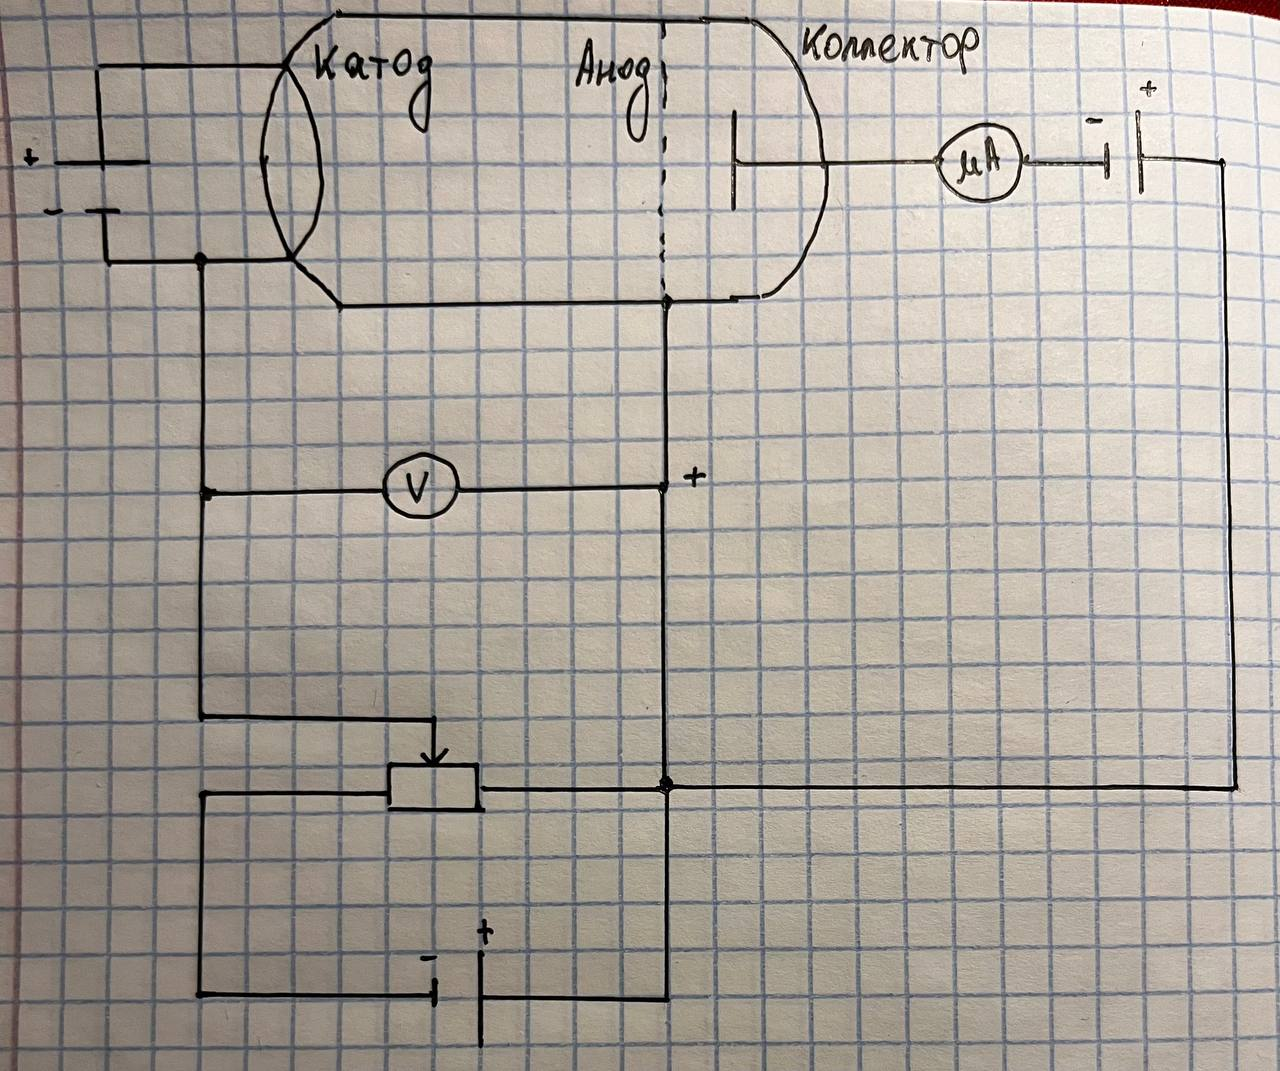
\includegraphics[scale=0.25]{hand1.jpg}
    \caption{Схема опыта Франка-Герца}
    \label{fig:vac}
\end{figure}

Опыт Франка-Герца подтверждает существование дискретных уровней энергии атомов. Разреженный одноатомный газ заполняет трёхэлектродную лампу. Электроны, испускаемые разогретым катодом, ускоряются в постоянном электрическом поле, созданном между катодом и сетчатым анодом лампы. Передвигаясь от катода к аноду, электроны сталкиваются с атомами гелия.

\begin{figure}[!h]
\begin{center}
\begin{minipage}[h]{0.45\linewidth}
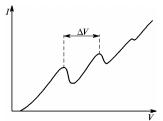
\includegraphics[width=1\linewidth]{fig2.PNG}
\caption{Схематический вид зависимости тока коллектора от напряжения на аноде}
\label{ris:experimcoded}
\end{minipage}
\end{center}
\end{figure}

Кинетическая энергия электрона 1 уровня равна:
\begin{equation}\label{key}
	E = \overline{e} \Delta V \left[\text{эВ}\right],
\end{equation}
где $ \Delta V $ -- разность между двумя пиками (см. рис. \ref{ris:experimcoded}).

\subsection{Описание установки}

На рис \ref{fig:vac} обозначены:
$A$ - амперметр; $\text{Б}7-4$ - стабилизированный источник питания (подаёт напряжение накала); $K_1$ - тумблер для включения в цепь источника $\text{Б}7-4$; $\text{Б}5-10$ - выпрямитель (подаёт на анод ускоряющее напряжение); $Pi_3$ - потенциометр, регулирующий величину ускоряющего напряжения; $V_1$ - вольтметр, измеряющий величину ускоряющего напряжения; 4.5 $B$ - батарея КБСЛ; $Pi_2$ - потенциометр, регулирующий величину задерживающего потенциала; $V_2$ - вольтметр, измеряющий величину задерживающего потенциала; $\mu A$ - микроамперметр; $K_3$ - ключ, переключающий схему из статического режима в динамический; Т - понижающий трансформатор - подаёт ускоряющий потенциал при динамическом режиме: 

\begin{figure}[!h]
    \centering
    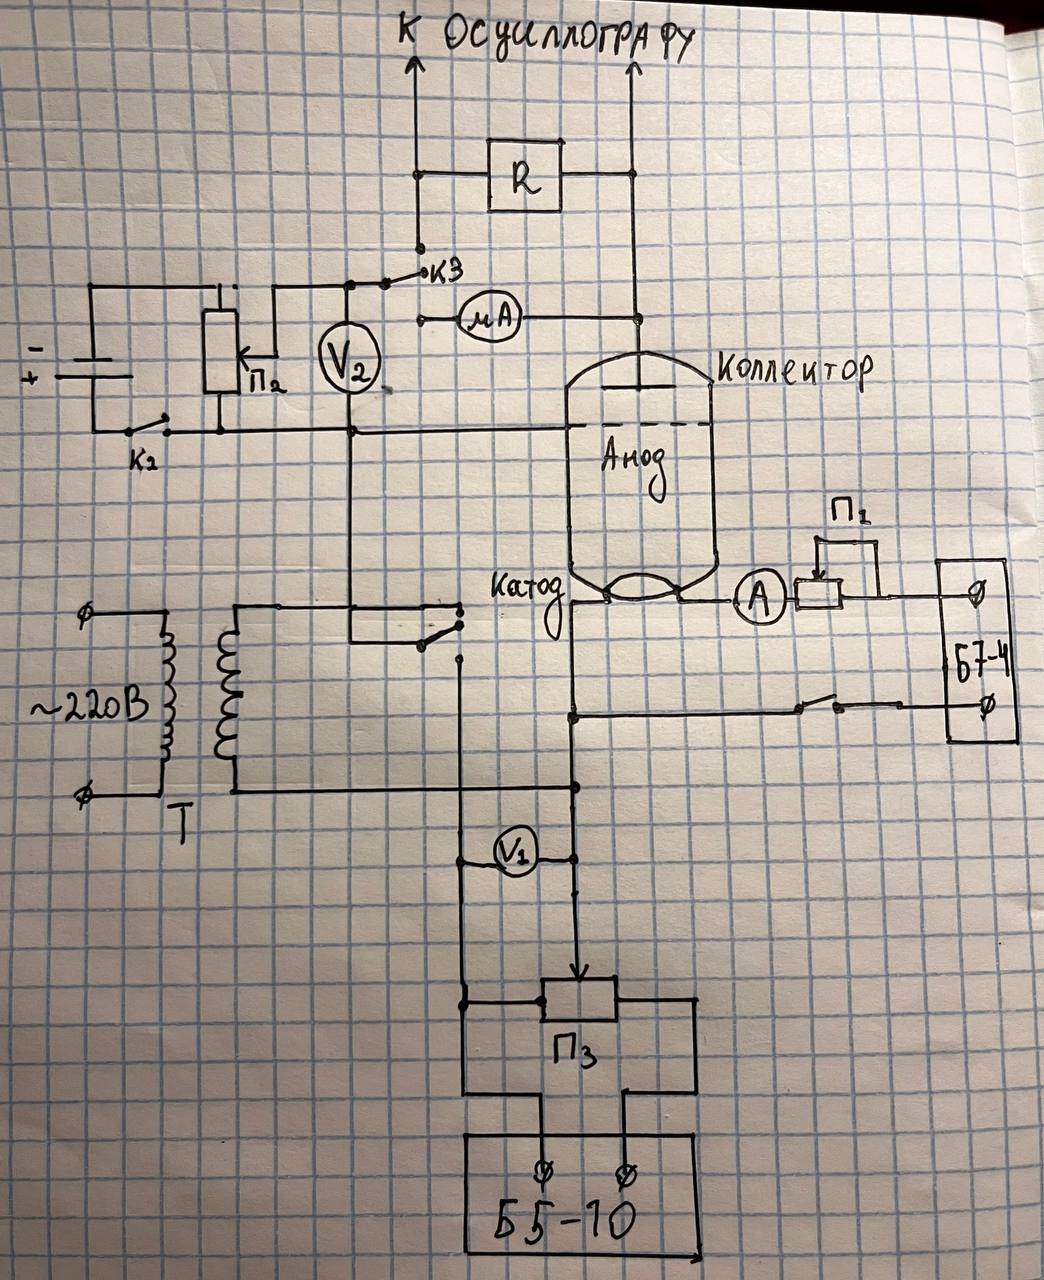
\includegraphics[scale=0.25]{hand2.jpg}
    \caption{Схема экспериментальной установки}
    \label{fig:vac}
\end{figure}

\newpage

\section{Ход работы}
\begin{itemize}

\item [\textbf{Динамика}] По расстоянию между соседними максимумами на осциллограммах определим энергию возбуждения первого уровня атома гелия в электрон-вольтах:

\begin{figure}[!h]
    \centering
    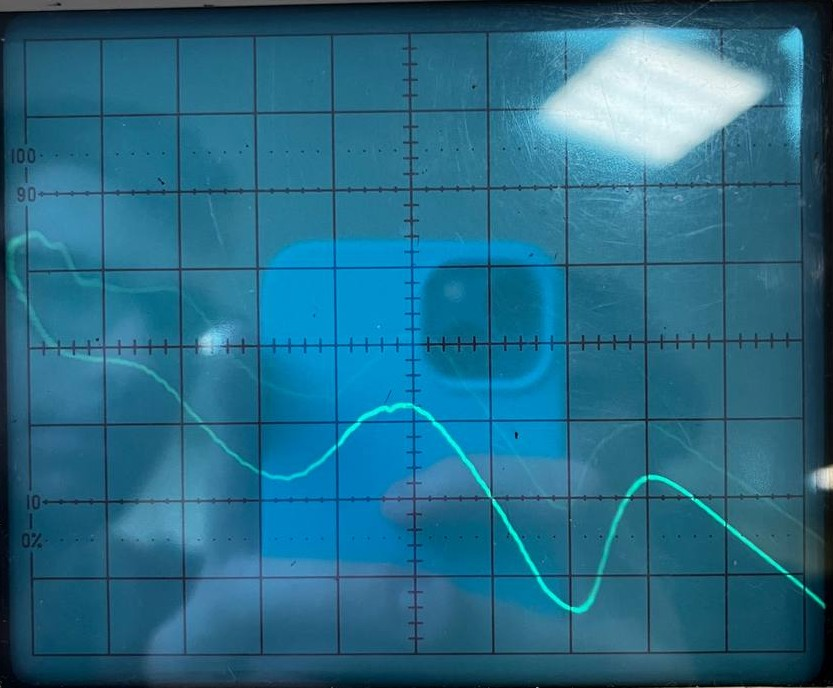
\includegraphics[scale=0.45]{graph1.jpg}
    \caption{График (динамика) $I_k(V_a)$ при $V_{\text{задер.}} = 4 B$}
    \label{graph:1}
\end{figure}

\newpage

\begin{figure}[!h]
    \centering
    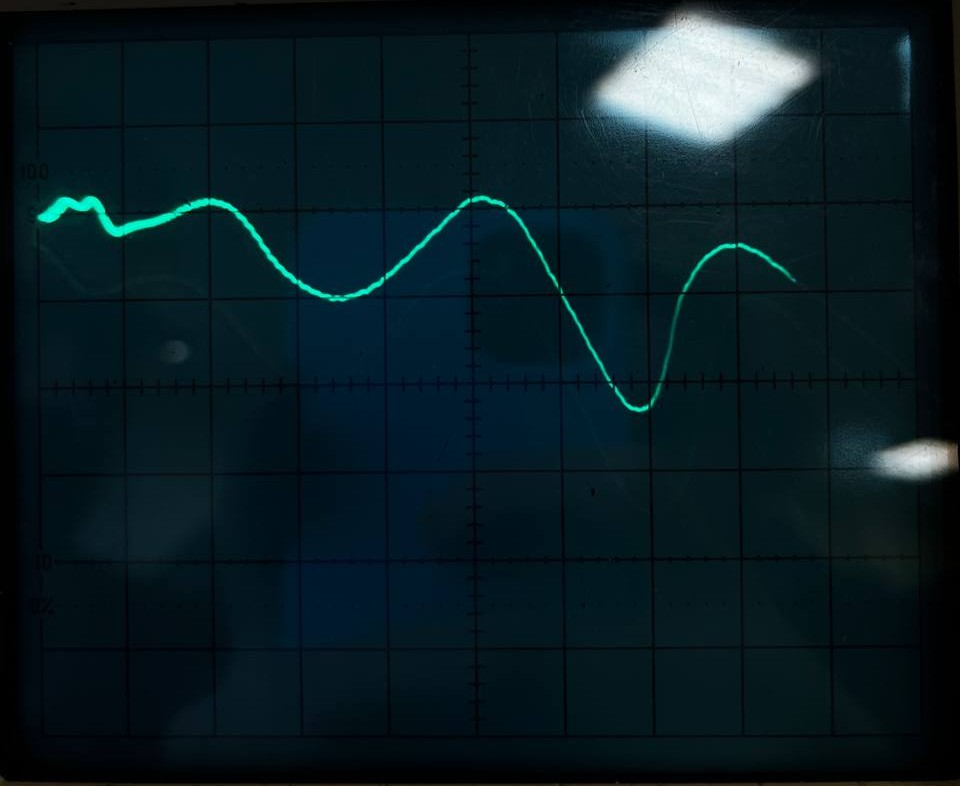
\includegraphics[scale=0.39]{graph2.jpg}
    \caption{График (динамика) $I_k(V_a)$ при $V_{\text{задер.}} = 6 B$}
    \label{graph:2}
\end{figure}

\begin{figure}[!h]
    \centering
    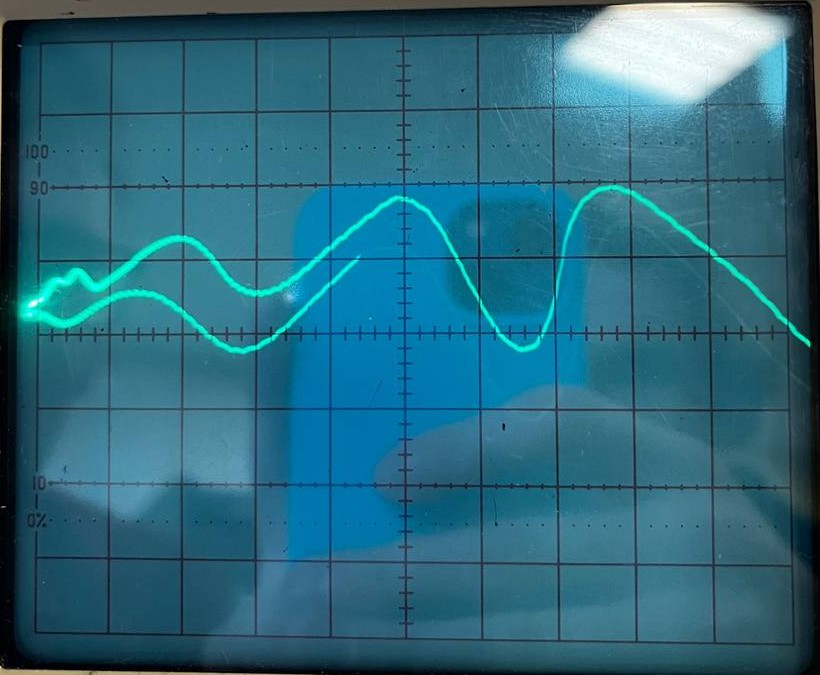
\includegraphics[scale=0.45]{graph3.jpg}
    \caption{График (динамика) $I_k(V_a)$ при $V_{\text{задер.}} = 8 B$}
    \label{graph:3}
\end{figure}

\newpage

Из графиков получим:

\begin{table}[!h]
\begin{center}
\begin{tabular}{|r|r|r|r|r|}
\hline $V_{\text{задер.}}$ & $\Delta V_{max\ 0-1}$& $\Delta V_{max\ 1-2}$ & $\Delta V_{min\ 0-1}$ & $\Delta V_{min\ 1-2}$ \\
\hline 4 & 14 & 15 & 17 & 12 \\
\hline 6 & 15 & 16 & 18 & 13 \\
\hline 8 & 14 & 15 & 19 & 12 \\
\hline
\end{tabular}
\end{center}
\caption{Расстояние между максимумами и минимумами (динамика)}

Рассчитаем среднее значение:
 		
 		\begin{equation*}
 			\Delta V = (15,0 \pm 3,5) \text{ В} \hspace{20mm} (\text{погрешность}\thicksim 23 \% )
 		\end{equation*}
 	
Тогда энергия возбуждения первого уровня для атома гелия:
 		\begin{equation*}
 			E_1 = (15,0 \pm 3,5) \text{ эВ} \hspace{20mm} (\text{погрешность}\thicksim 23 \% )
 		\end{equation*}


\label{tab1}
\end{table}

\item  [\textbf{Статика}] Построим графики $I_{\mathrm{K}}=f\left(V_{\mathrm{a}}\right)$ при $V_{\text{задер.}}=$ const. По графикам определим энергию возбуждения первого уровня атома гелия (все значения в файле $Data.xlsx$):

\begin{figure}[!h]
    \centering
    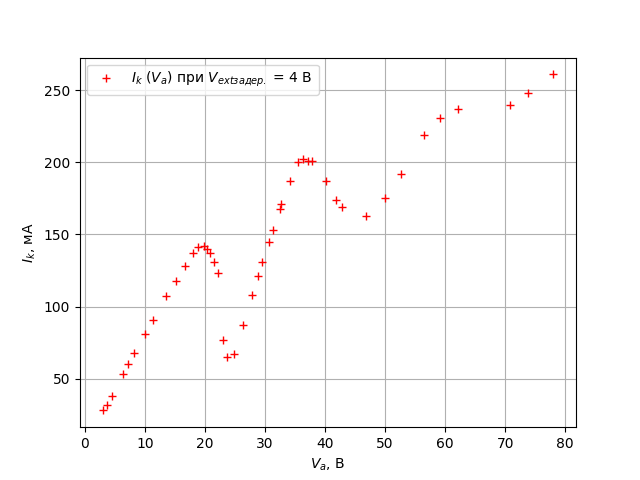
\includegraphics[scale=0.55]{graph4.png}
    \caption{График (статика) $I_k(V_a)$ при $V_{\text{задер.}} = 4 B$}
    \label{graph:4}
\end{figure}

\begin{figure}[!h]
    \centering
    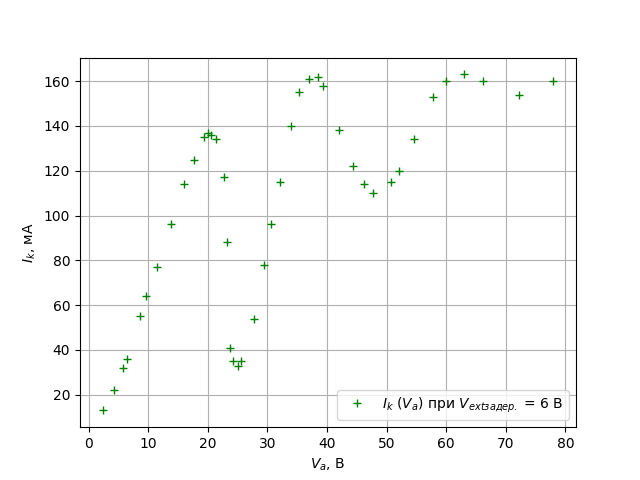
\includegraphics[scale=0.55]{graph5.png}
    \caption{График (статика) $I_k(V_a)$ при $V_{\text{задер.}} = 6 B$}
    \label{graph:5}
\end{figure}

\newpage

\ 

\begin{figure}[!h]
    \centering
    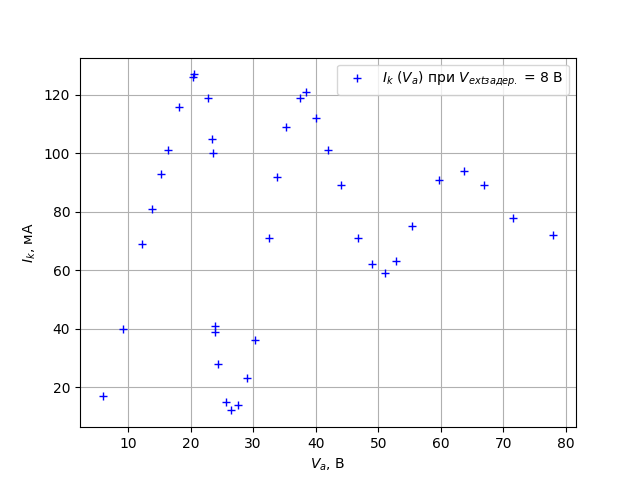
\includegraphics[scale=0.55]{graph6.png}
    \caption{График (статика) $I_k(V_a)$ при $V_{\text{задер.}} = 8 B$}
    \label{graph:6}
\end{figure}

\begin{figure}[!h]
    \centering
    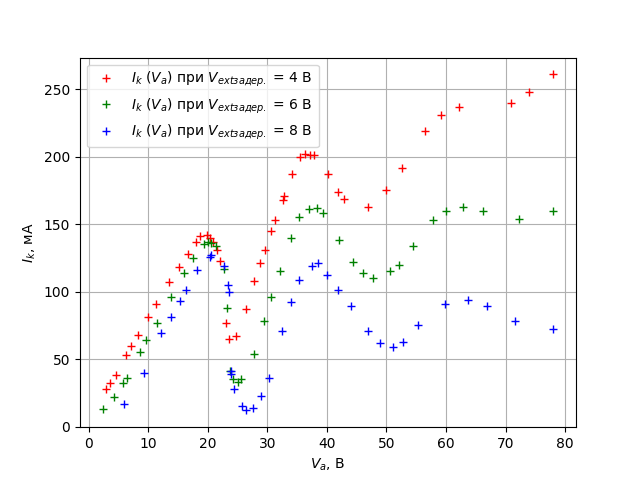
\includegraphics[scale=0.55]{all.png}
    \caption{График (статика) $I_k(V_a)$ для всех значений $V_{\text{задер.}}$}
    \label{graph:all}
\end{figure}

\ $\text{ }$

\begin{table}[!h]
    \centering
    \begin{center}
    \caption{Максимумы и минимумы напряжения на осциллограммах}
    \end{center}
    \vspace{0.1cm}
    \label{tab:my_label}
    \begin{tabular}{ |p{3.5cm}||p{1.5cm}|p{1.5cm}|p{1.5cm}|p{1.5cm}|p{1.5cm}|p{1.5cm}|}
 \hline
$V_{\text{задер.}}$ & $V_{max_1}$ & $V_{max_2}$ & $V_{min_1}$ & $V_{min_2}$  & $\triangle V_{max}$ & $\Delta V_{min}$\\
 \hline
 4 В & 23.76 В & 39.26 В & 25.41 В & 49.34 В  & 15.5 В & 23.93 В\\
\hline
 6 В & 23.82 В & 36.68 В & 24.78 В & 48.29 В  & 12.86 В & 23.51 В\\
\hline
 8 В & 25.33 В & 38.75 В & 25.62 В & 50.40 В  & 13.42 В & 24.78 В\\
\hline

\end{tabular}
\end{table} 

\newpage


Для $V_{\text{задер.}} = 4B$:
 		\begin{equation*}
 			\Delta V = (21,72 \pm 0,07) \text{ В}
 			\hspace{20mm} (\text{погрешность}\thicksim 0,32 \% )
 		\end{equation*}
Для $V_{\text{задер.}} = 6B$:
  		 		\begin{equation*}
 			\Delta V = (21,89 \pm 0,09) \text{ В}
 			\hspace{20mm} (\text{погрешность}\thicksim 0,41 \% )
 		\end{equation*}
 		
Для $V_{\text{задер.}} = 8B$:
 		\begin{equation*}
 			\Delta V = (22,0 \pm 0,2) \text{ В}
 			\hspace{20mm} (\text{погрешность}\thicksim 0,91 \% )
 		\end{equation*}
 	
Усредним энергию возбуждения первого уровня атома гелия для 3х значений $V_{\text{задер.}}$:
 		\begin{equation*}
 			\Delta V^\Sigma = (21,9 \pm 0,3) \text{ В}
 		\end{equation*}
 	
 		А значит, энергия возбуждения первого уровня атома гелия равна:
 		\begin{equation*}
 			E_1^\Sigma = (21,9 \pm 0,3) \text{ эВ}
 			\hspace{20mm} (\text{погрешность}\thicksim 1,40 \% )
 		\end{equation*}
 	



\item  [3.] Сравним результаты измерений, полученные при динамическом и статическом методах измерений:

Значения, полученные при помощи динамического и статического метода сильно различаются, как и погрешности полученных значений.
 	

\item  [4.] Теперь оценим достоверность полученных результатов (т.е. сравним с табличными данными):

Статический оказался лучше (ближе к теоретическому значению и с меньшей погрешностью), нежели динамический.

\end{itemize}

\newpage

\section{Вывод}

В ходе выполнения опыта Франка-Герца мы проверили утверждение о наличии дискретных уровней возбуждения атомов. Опыт проводился в 2х режимах:

\begin{itemize}
 		\item [\textbf{dynamic}]$E = (15,0 \pm 3,5) \text{ эВ} \hspace{20mm} (\text{погрешность}\thicksim 23 \% )$
 		
 		\item [\textbf{static}]$E = (21,9 \pm 0,3) \text{ эВ} \hspace{20mm} (\text{погрешность}\thicksim 1,4 \% )$
 	\end{itemize}

Сравнивая полученные результаты с табличным значением ($E = 21,6 \text{ эВ}$) получили, что статический метод дал близкое (в пределах $\sigma$) значения к теоретическому, в то время как динамический попал в пределы $2\sigma$, да и сама $\sigma$ большая.

Причины таких ошибок:

\begin{itemize}
 		\item [\textbf{dynamic}] Методика снятия данных имеет большую погрешность, т.к. цена деления осциллографа была $5V$.
 		
 		\item [\textbf{static}] Такая маленькая (по сравнению с динамическим) погрешность обусловленна тем, что у вольтметра и амперметра погрешности на пару порядков меньше, чем у осциллографа.
 	\end{itemize}
 	

\section{Литература}

\begin{enumerate}

\item Лабораторный практикум по общей физике. Квантовая физика.

\item МНК -- http://mathhelpplanet.com/static.php?p=onlayn-mnk-i-regressionniy-analiz

\end{enumerate}	

\end{document}
